\documentclass[10pt,a4paper]{article}
\usepackage[utf8]{inputenc}
\usepackage{amsmath}
\usepackage{amsfonts}
\usepackage{amssymb}
\usepackage{graphicx,longtable,mathrsfs,color}
\usepackage{epsfig,subfigure,placeins,float} % plots
\usepackage[usenames,dvipsnames]{xcolor} % colour
\title{Notes: Error on the Power Spectrum}
\author{Sahba Yahya}
\begin{document}

\maketitle


\section{Analytic solution }
\begin{eqnarray}\label{FIJ_DEV}
F_{ij}^*&=& V_{\rm sur} \int_{k_{min}}^{K_{max}} \frac{ 2 \pi k^2 dk}{2 (2 \pi)^3} \left[1+\frac{1}{nP}\right]^2
\end{eqnarray}

where,
\begin{eqnarray}
P(k,\mu)&=& R(\mu,k)P_{lin}(k) \left[\frac{g(z)}{g(z_{in})} \frac{(1+z_{in})}{(1+z)}\right]^2 b^2,\\
R(\mu,k)& =&1.\label{eq:Rsig}
\end{eqnarray}
and
\begin{equation}\label{Vsurvey}
V_{\rm sur} = \left(\frac{\pi}{180}\right)^2 \ S_{\rm area}\int^{z_{\rm min}}_{z_{\rm max}} \frac{dV}{dz}, 
\end{equation}
where $z_{\rm min} = 0. 9 $,  $z_{\rm max} = 1.1 $ and $S_{\rm area} = 30000 \  {\rm deg}^2$. $dV/dz$ defined as:\[dV/dz=  (1+z)^2D_A^2 \frac{c }{H_0} \frac{1}{h}\]
The units for the $V_{\rm sur}$ is $h^{-3} {\rm Mpc}^3$.

Setting $ n \sim \infty$ 
\begin{equation}
F_{ij}^*= V_{\rm sur} \int_{k_{min}}^{K_{max}}  \frac{ 2 \pi k^2 dk}{2 (2 \pi)^3}
\end{equation}

solve the integral 
\begin{equation}\label{dp_ov_p}
F_{ij}^*= V_{sur} \frac{1}{ (24 \ \pi^2 )} \left[ k_{max}^3 -k_{min} ^3 \right]
\end{equation}

Arbitrary choices, $k_{min} = 0.001$, $k_{max} = 0.1$ and $V_{\rm sur} = 3{\rm e}10$ for z=1, and survey area is 30000 [deg$^2$]:

\begin{equation}
F_{ij}^* = 5.25512 \times 10^{-7}  V_{\rm sur}   = 8554,
\end{equation}
\begin{equation}
\frac{\delta P}{P} = \sqrt{(F_{ij}^*)^{-1}} = 0.011,
\end{equation}
Fig.~\ref{fig:cosmic_limit} shows $\frac{\delta P}{P}$ for $S_{rms} = 7.3$ and  the analytic solution proven above.
%====================================
\section{Euclid}

 Fig.~\ref{fig:cosmic_limit_Euclid_1} shows Euclid $\frac{\delta P}{P}$ produced using the definition in Bull et al 2014, not this figure shows produced with z =1, the bias = $ \sqrt{(1+z)}$ =1.41421, $k_{\rm max} = 0.16926\  h {\rm Mpc}^{-1}$, the survey volume has been calculated using Eq.~\ref{Vsurvey} and the Survey area is 15000 deg$^2$.



Fig.~\ref{fig:cosmic_limit_Euclid_2} shows the binned $k$ $\rm{Mpc}^{-1}$h. To check with Phil Bull results, we run camb with Plank's best fit parameters (see Fig.~ \ref{fig:pk_vs_k}):

\begin{verbatim}
# Planck best-fit parameters
cosmo = {
    'omega_M_0':        0.316,
    'omega_lambda_0':   0.684,
    'omega_b_0':        0.049,
    'N_eff':            3.046,
    'h':                0.67,
    'ns':               0.962,
    'sigma_8':          0.834,
    'gamma':            0.55,
    'w0':               -1.,
    'wa':               0.,
    'sigma_nl':         7.,
\end{verbatim}
%The surprising thing and I don't understand is the breakage on the non-binned $\delta p/p$ (the problem solved!)

%================================================
\section{Fractional error on DA and H}
Fig.~\ref{fig:lnda_lnH} shows the errors on $\sigma_H/H \%$ and  $\sigma_{D_A}/D_A \%$ using wiggles only method.



\begin{figure}
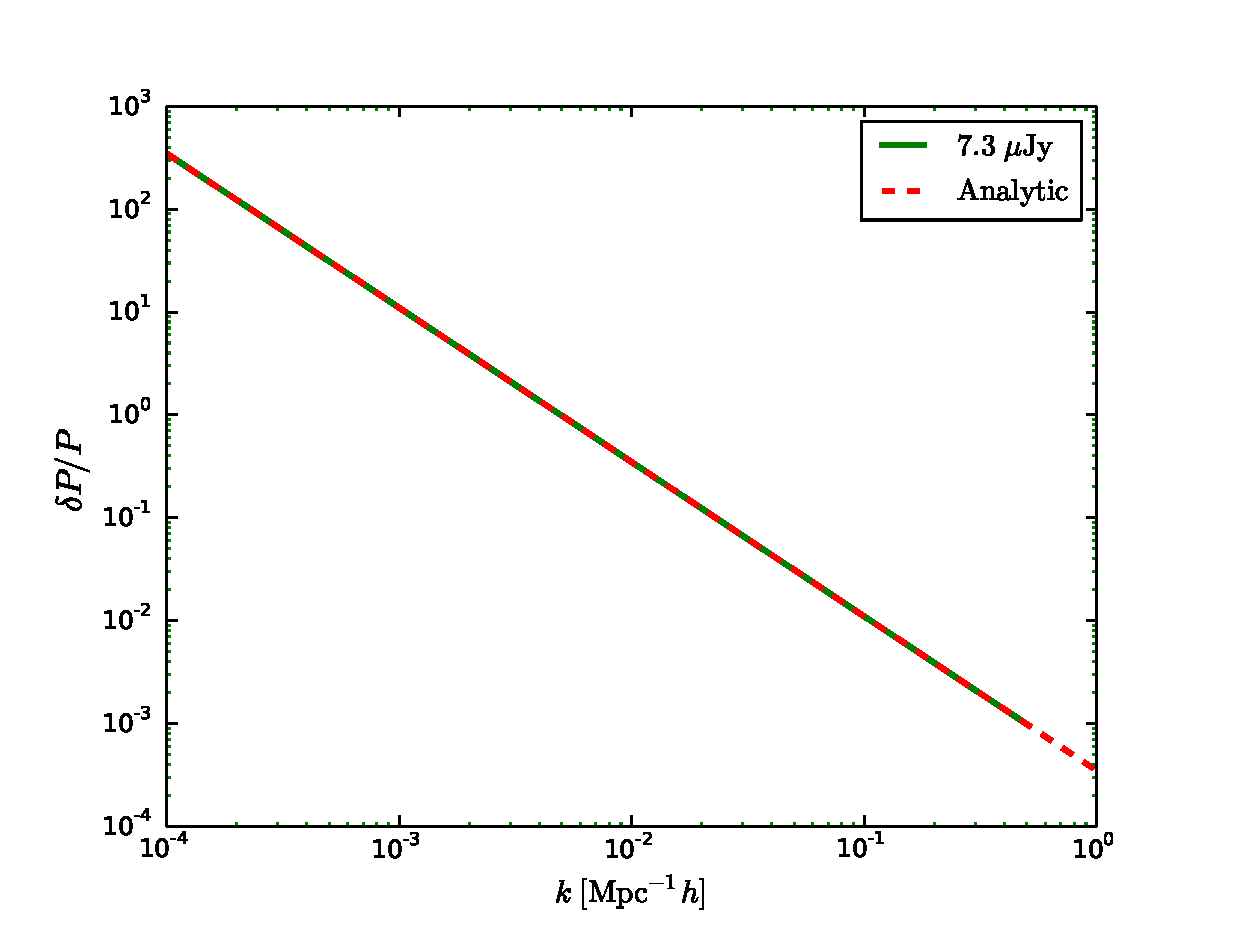
\includegraphics[width=1.0\textwidth]{deltaP_ov_p.eps}
\caption{The Figure shows $\delta P/P$ where n is very large (using Eq.~\ref{dp_ov_p}). The red dot point represent the analytic solution, for red-shift 1 and the corresponding bias=1.4.}
\label{fig:cosmic_limit}

\end{figure}



\begin{equation}
\left( \frac{\delta P}{P} \right)^2 =\left[ V_{\rm sur} \int_{k_{min}}^{K_{max}} \frac{ 2 \pi k^2 dk}{2 (2 \pi)^3} \left(1+\frac{1}{nP}\right)^2\right]^{-1}
\end{equation}



\begin{figure}
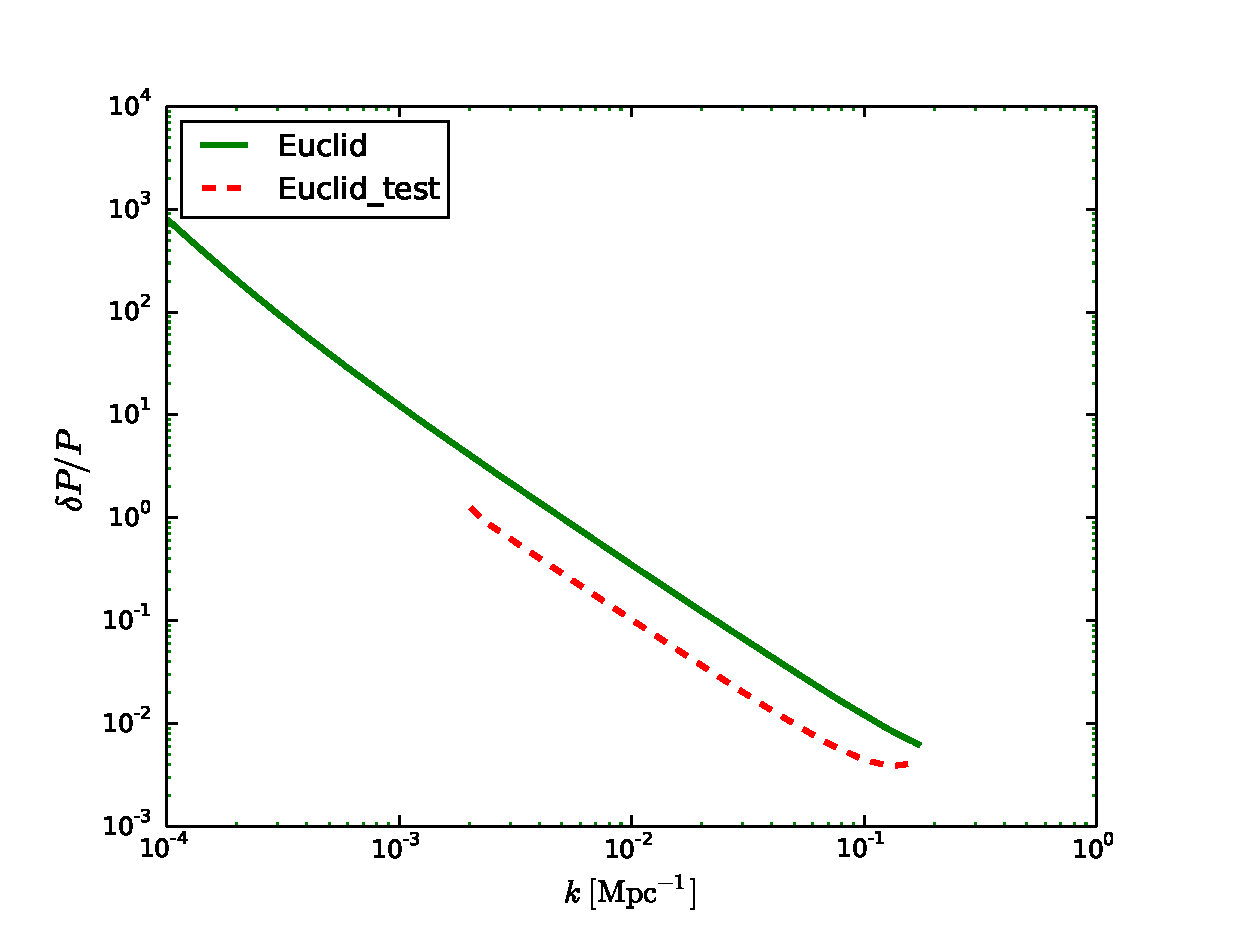
\includegraphics[width=1.0\textwidth]{deltaP_ov_p_Euclid_2.eps}
\caption{The Figure shows $\delta P/P$  for Euclid, for red-shift 1 and the corresponding bias=1.5.}
\label{fig:cosmic_limit_Euclid_1}
\end{figure}

\begin{figure}
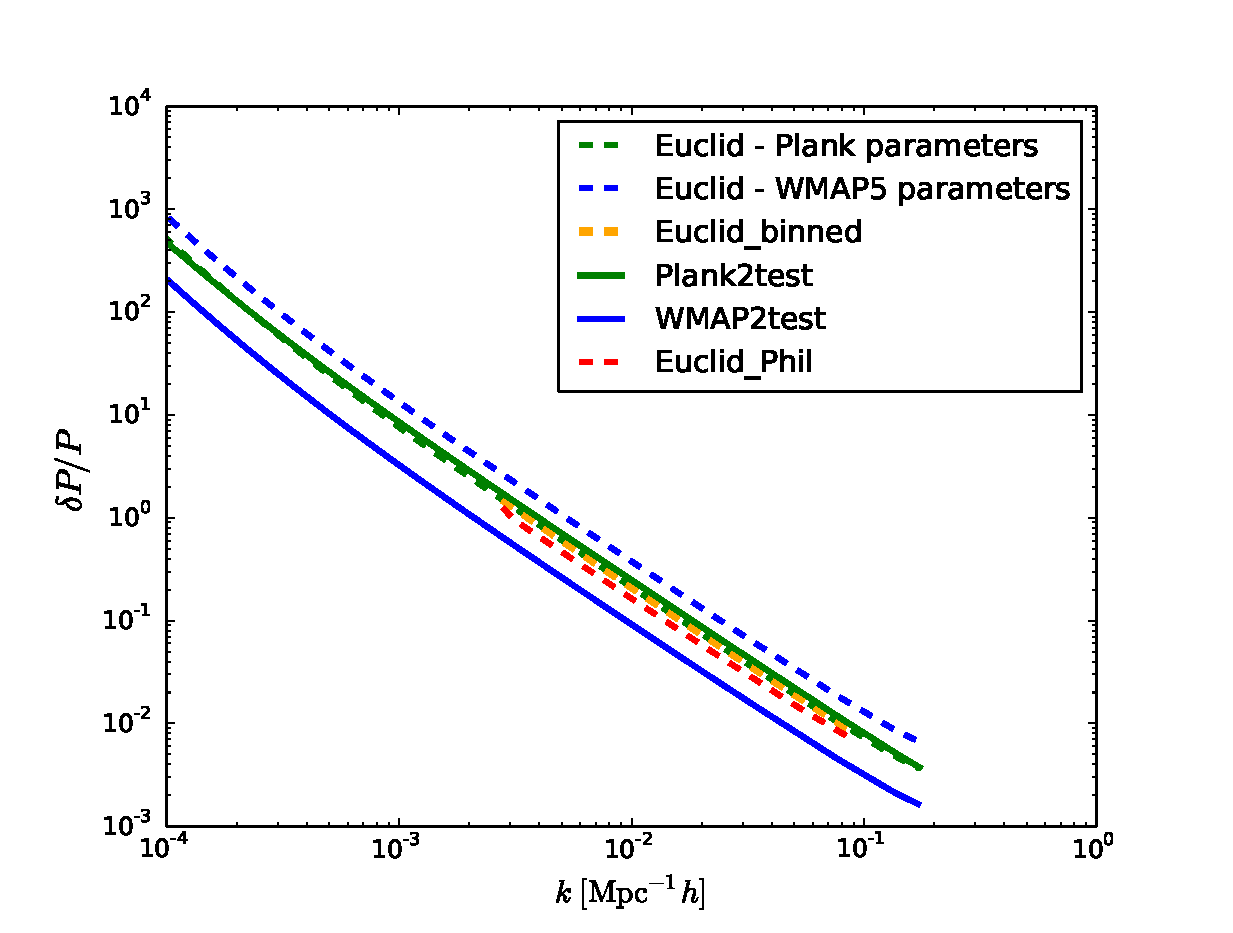
\includegraphics[width=1.0\textwidth]{deltaP_ov_p_Euclid.eps}
\caption{The Figure shows $\delta P/P$  for Euclid, for red-shift 1 and the corresponding bias=1.5. All the approached lie on top of each other except when we use the WMAP 5 parameters (blue).}
\label{fig:cosmic_limit_Euclid_2}
\end{figure}

\begin{figure}
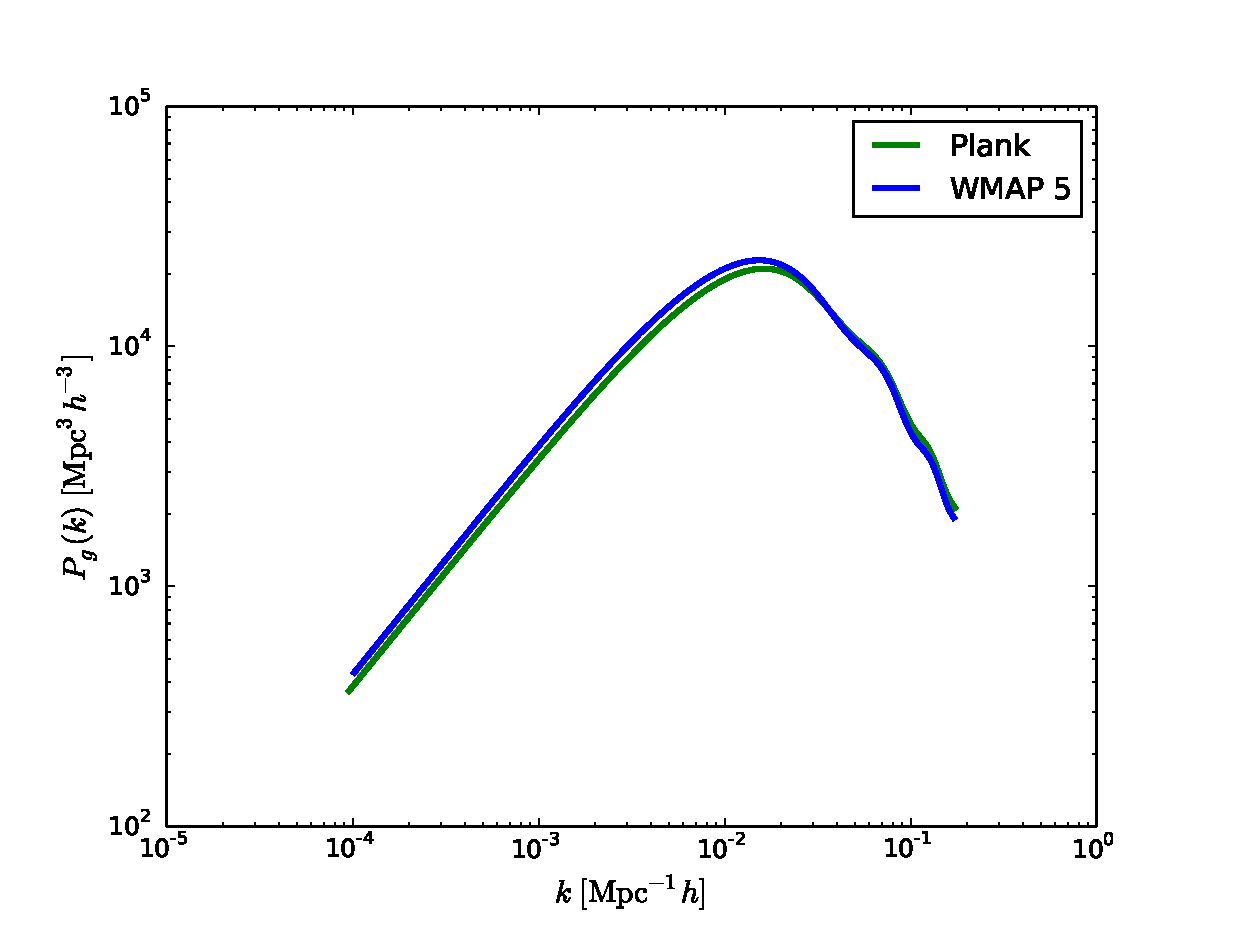
\includegraphics[width=1.0\textwidth]{pk.eps}
\caption{The power spectrum vs $k$ Mpc$h^{-1}$}
\label{fig:pk_vs_k}
\end{figure}
 

\begin{figure}
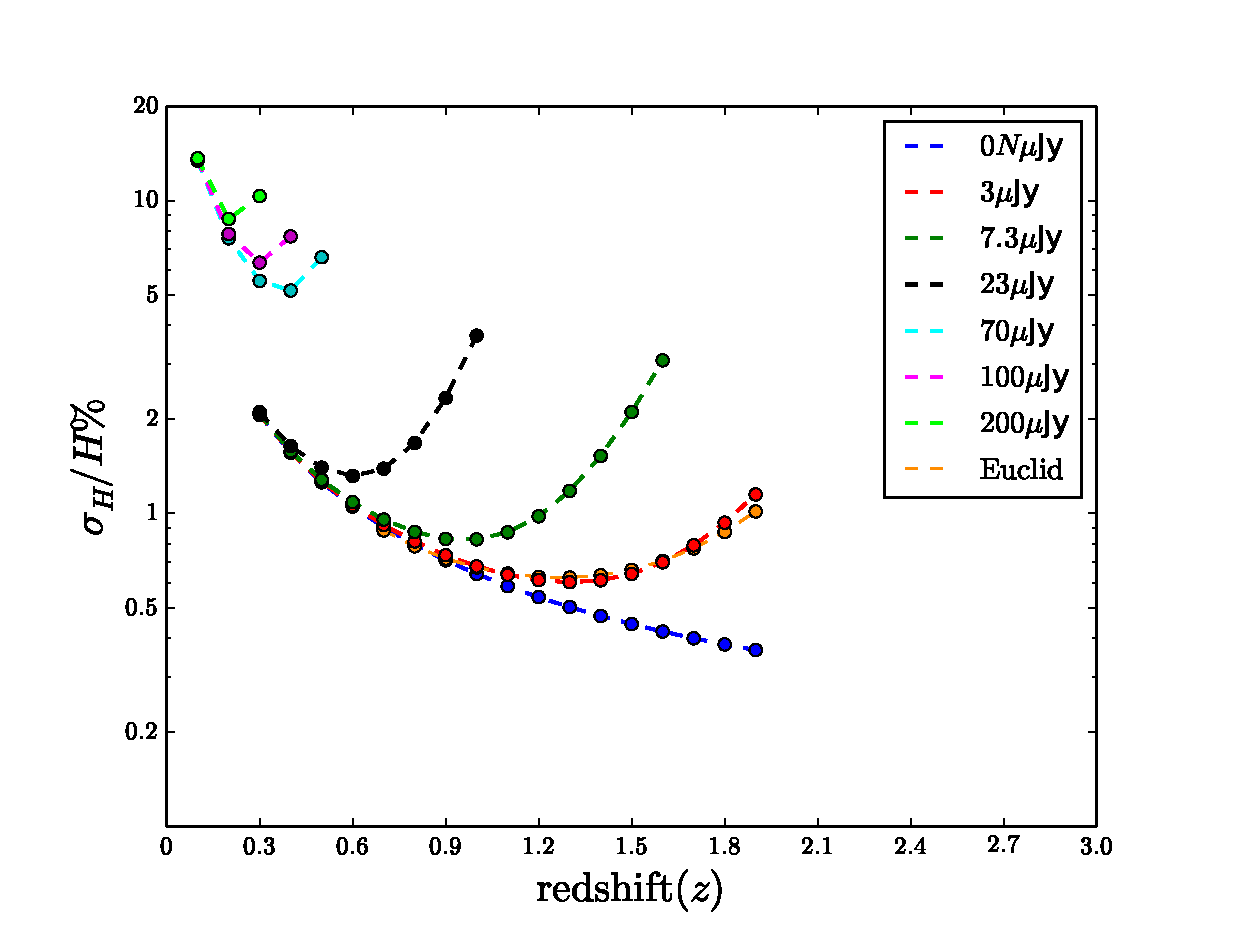
\includegraphics[width=1.0\textwidth]{output_lnH_mario_bias.eps}
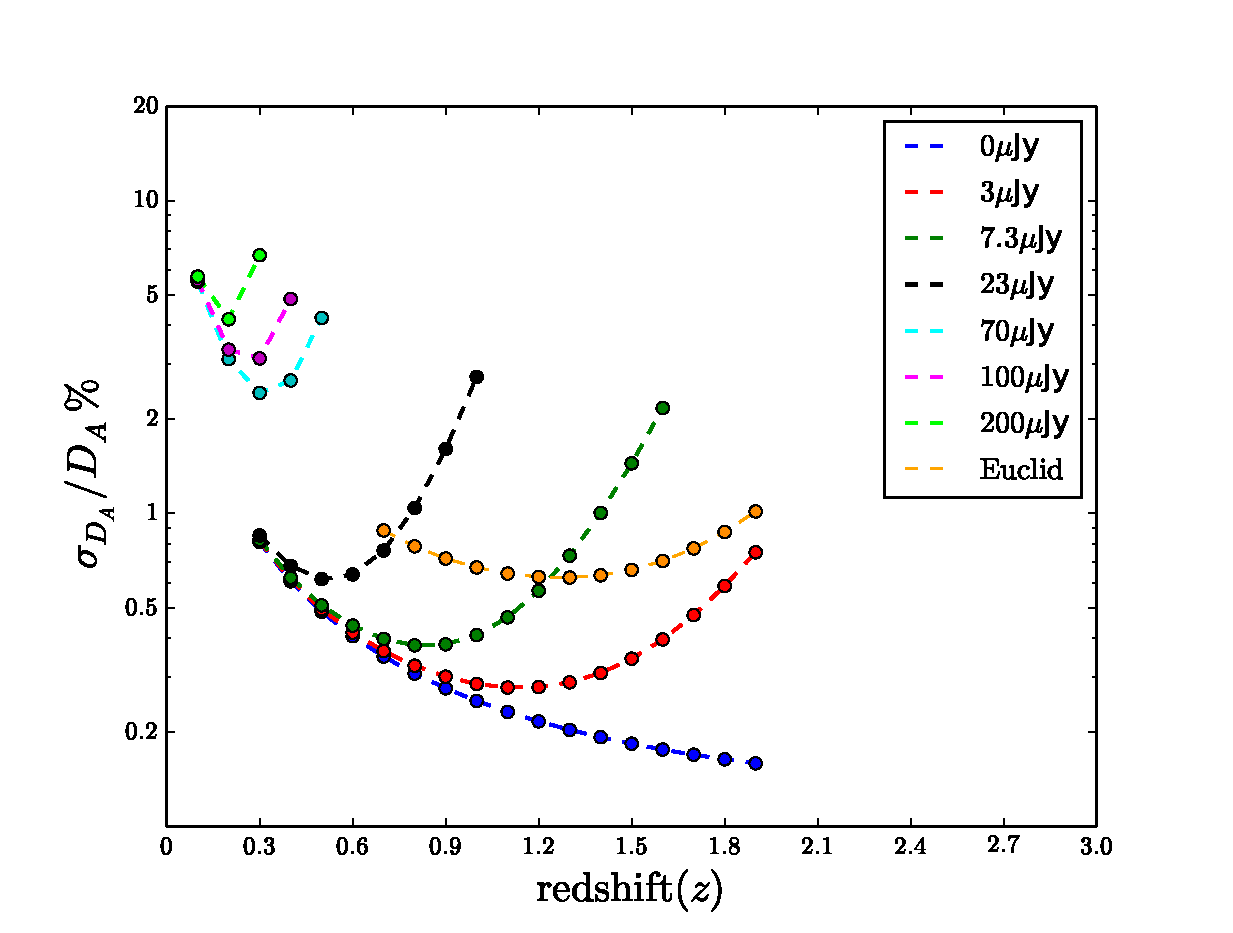
\includegraphics[width=1.0\textwidth]{output_lnda_mario_bias.eps}
\caption{The Figure shows $\sigma_H/H \%$ and $\sigma_{D_A}/D_A \%$  for SKA and  Euclid (orange).}
\label{fig:lnda_lnH}
\end{figure}


\section{Binning the Power spectrum}

Binning primary goal is to reduce the effects of minor observation errors. The original data values which fall in a given small interval (bin) replaced by a value usually in the middle of that interval. 

Combining Eq.~\ref{Vsurvey} and Eq.~\ref{dp_ov_p}  and replacing $k_{\rm min}$ and $k_{\rm max}$ by $k$ and $k+ \Delta k$ respectively, we get:
\begin{equation}\label{dp_ov_p}
F_{ij}^*= V_{sur} \frac{1}{ (24 \ \pi^2 )} \left[ k^3 -(k+ \Delta k) ^3 \right]
\end{equation}
\begin{equation}\label{dp_ov_p_deltak}
F_{ij}^*= V_{sur} \frac{1}{ (24 \ \pi^2 )} \left[ 2 k^3 + 3k^2  \Delta k  + 3 k \Delta k^2 + \Delta k^3 \right]
\end{equation}

Choosing the size and the width of the bin is essential, from Eq.~\ref{dp_ov_p_deltak}, choosing wider bins will make $\delta p/p$ smaller than choosing finer bins.

\section{Baryon Power spectrum}






\end{document}